\section{问题一模型建立与求解}

\subsection{问题一分析}

问题一以附件1的单日负载、光伏和电价为确定输入，在零时联合安排144个10分钟时段的购电与储能动作，并将日末库存恢复至日初水平。参照日前微网调度研究\cite{kong2016,silva2020}构建线性规划，依据价差、效率、容量及后续补能机会分配电量，为后续各问提供共同物理基础。

\subsection{问题一模型建立}

\begin{modelsummary}{问题一模型汇总}
\textbf{输入：}单日负载与光伏功率、分时电价、电池效率及库存边界，按十分钟换算为电量。\par
\textbf{决策：}144段购电、充放电与储电量。\par
\textbf{目标：}最小化按计划量全额结算的外购电费。\par
\textbf{约束与输出：}供给不低于需求，遵循储能递推、效率及功率容量界，首末库存均为6000 kWh；输出购电计划、充放电轨迹、四小时电量汇总和全日费用。
\end{modelsummary}

\subsubsection{决策变量与购电目标}

按统一物理索引$t=0,\ldots,143$，定义计划购电$g_t$、电池外侧充电$c_t$、电池外侧放电$d_t$和时段初储电量$e_t$，单位均为kWh。净负荷为$n_t=(L_t-R_t)\Delta t$，可以为负，负值表示光伏超过当期负载。购电按时段电价$p_t$收费，因此目标为
\begin{equation}
 \min_{g,c,d,e}\quad C_1=\sum_{t=0}^{143}p_tg_t.
 \label{eq:q1_objective}
\end{equation}
功率先乘$\Delta t=1/6$ h得到电量，故费用直接按$p_tg_t$计算。目标计入外购电费，富余电量可免费弃置。

\subsubsection{供需、储能与日末约束}

在任一时段，外网采购与电池放电至少补足净负荷及充电需求：
\begin{equation}
 g_t+d_t-c_t\ge n_t.
 \label{eq:balance}
\end{equation}
令$w_t=g_t+d_t-c_t-n_t\ge0$，即可改写为电量平衡等式，其中$w_t$为免费弃置的富余量。

电池状态沿时间传递：
\begin{equation}
 e_{t+1}=e_t+\eta_cc_t-\frac{d_t}{\eta_d},
 \qquad \eta_c=\eta_d=0.9.
 \label{eq:soc}
\end{equation}
充电量$c_t$在电池外侧计量，$0.9c_t$进入电池；对外输出$d_t$需消耗内部电量$d_t/0.9$，往返效率为0.81。

容量和功率约束为
\begin{equation}
 E_{\min}\le e_{t+1}\le E_{\max},\qquad
 0\le c_t,d_t\le U,
 \quad E_{\min}=1200,\quad E_{\max}=10800,\quad U=5000/6.
 \label{eq:limits}
\end{equation}
储电量下限防止过度放电，上限防止过度充电；$U$由5000 kW乘$1/6$小时得到，分别限制一个时段可输入、输出的外侧电量。另有
\begin{equation}
 g_t\ge0,\qquad e_0=e_{144}=6000.
 \label{eq:terminal_q1}
\end{equation}
非负购电对应单向购入，首末相等使单日调度保持库存中性。上述线性目标与约束可直接作为LP求解。

\subsubsection{免费弃余条件下的充放电互斥证明}

免费弃余条件下，连续变量LP即可获得充放电互斥的最优解。若某可行解在时段$t$有$c_t,d_t>0$，取
\begin{equation}
 \varepsilon=\min\{c_t,d_t/(\eta_c\eta_d)\},\qquad
 c'_t=c_t-\varepsilon,\quad
 d'_t=d_t-\eta_c\eta_d\varepsilon.
 \label{eq:q1_remove_simultaneous}
\end{equation}
变换后至少一种动作变为零，充放电量均缩减且保持非负，满足原功率界。同时
\[
 \eta_cc'_t-d'_t/\eta_d=\eta_cc_t-d_t/\eta_d,
\]
故全部储电轨迹与首末约束保持不变。供需约束左端增加$(1-\eta_c\eta_d)\varepsilon\ge0$，可将新增富余弃置，原购电量及费用无须增加。对所有同时充放电时段依次变换，得到满足互斥且费用不高于原解的方案。因此至少存在一组充放电互斥的最优解，无需为该条件额外引入整数变量。

程序在充放电总量上加入$10^{-7}$元/kWh的数值破同解项以减少循环，实际费用统计剔除该项。

\subsubsection{跨时段储能的经济条件}

若低价时段从外网购电并储存，要在高价时段对外输出1 kWh，低价段需购入$1/(\eta_c\eta_d)$ kWh。因此在忽略容量、功率及其他机会成本时，纯购电套利的必要盈利条件为
\begin{equation}
 p_h>\frac{p_\ell}{\eta_c\eta_d}=\frac{p_\ell}{0.81}.
 \label{eq:arbitrage}
\end{equation}
该式解释低价补能、高价替代购电的动机。完整LP还同时考虑容量的机会价值与终值要求：预期午间光伏可充满电池时，凌晨充电会占用其容量；临近日末则须为6000 kWh终值补能。

\subsection{问题一求解}

\subsubsection{求解步骤与结果核对}

按统一时间映射将附件1功率换算为电量，以式\eqref{eq:soc}组装稀疏状态约束，加入容量、功率和首末条件后由HiGHS求解。基于原精度结果核对144段供需、储电递推及动作可行性，再按同一物理索引生成费用、正文数表和工作簿。

计算得到全天计划购电量59482.6990 kWh、购电费35126.9486元。无储能基准逐时购买$[n_t]_+$，费用为48052.05元，因此采用储能节省12925.10元，节费率为26.90\%。电池外侧累计充电20740.67 kWh、放电16799.94 kWh，满足
\[
 \eta_c\sum_tc_t=\sum_td_t/\eta_d,
\]
与$e_0=e_{144}=6000$ kWh一致，外侧累计充放电量的差额对应效率损耗。

\begin{table}[htbp]\centering\small\caption{问题1指定时段与全天购电结果（电量单位：kWh）}\label{tab:q1-purchase}\begin{tabularx}{\linewidth}{lRlRlR}
\toprule
时间段 & 购电量 & 时间段 & 购电量 & 时间段 & 购电量\\
\midrule
10:00--10:10 & 0.00 & 12:00--12:10 & 480.41 & 14:00--14:10 & 0.00\\
16:00--16:10 & 445.43 & 18:00--18:10 & 531.89 & 20:00--20:10 & 0.00\\
\midrule
全天购电量 & 59482.70 & \multicolumn{2}{c}{全天购电费（元）} & \multicolumn{2}{r}{35126.95}\\
\bottomrule
\end{tabularx}\end{table}
\begin{table}[htbp]\centering\small\caption{问题1储能充放电及首末电量（单位：kWh）}\label{tab:q1-battery}\begin{tabularx}{\linewidth}{lRRlRR}
\toprule
时间段 & 充电量 & 放电量 & 时间段 & 充电量 & 放电量\\
\midrule
00:00--04:00 & 4500.00 & 0.00 & 04:00--08:00 & 833.33 & 6365.84\\
08:00--12:00 & 4787.96 & 1703.00 & 12:00--16:00 & 5286.04 & 91.10\\
16:00--20:00 & 0.00 & 5780.13 & 20:00--24:00 & 5333.33 & 2859.87\\
\midrule
0:00储电量 & \multicolumn{2}{r}{6000.00} & 24:00储电量 & \multicolumn{2}{r}{6000.00}\\
\bottomrule
\end{tabularx}\end{table}

表\ref{tab:q1-purchase}汇总为负载和储能安排的全部外购电，表\ref{tab:q1-battery}按六个物理四小时区间累计充放电。区间内两项均为正时，对应其中不同10分钟时段的互斥动作。

\subsubsection{调度结构与能量收支}

图\ref{fig:q1}对齐展示购电、充放电、SOC及电价，呈现电池随价格和净需求变化转移电量的过程。曲线保留原始LP的分段动作。

\begin{figure}[htbp]\centering
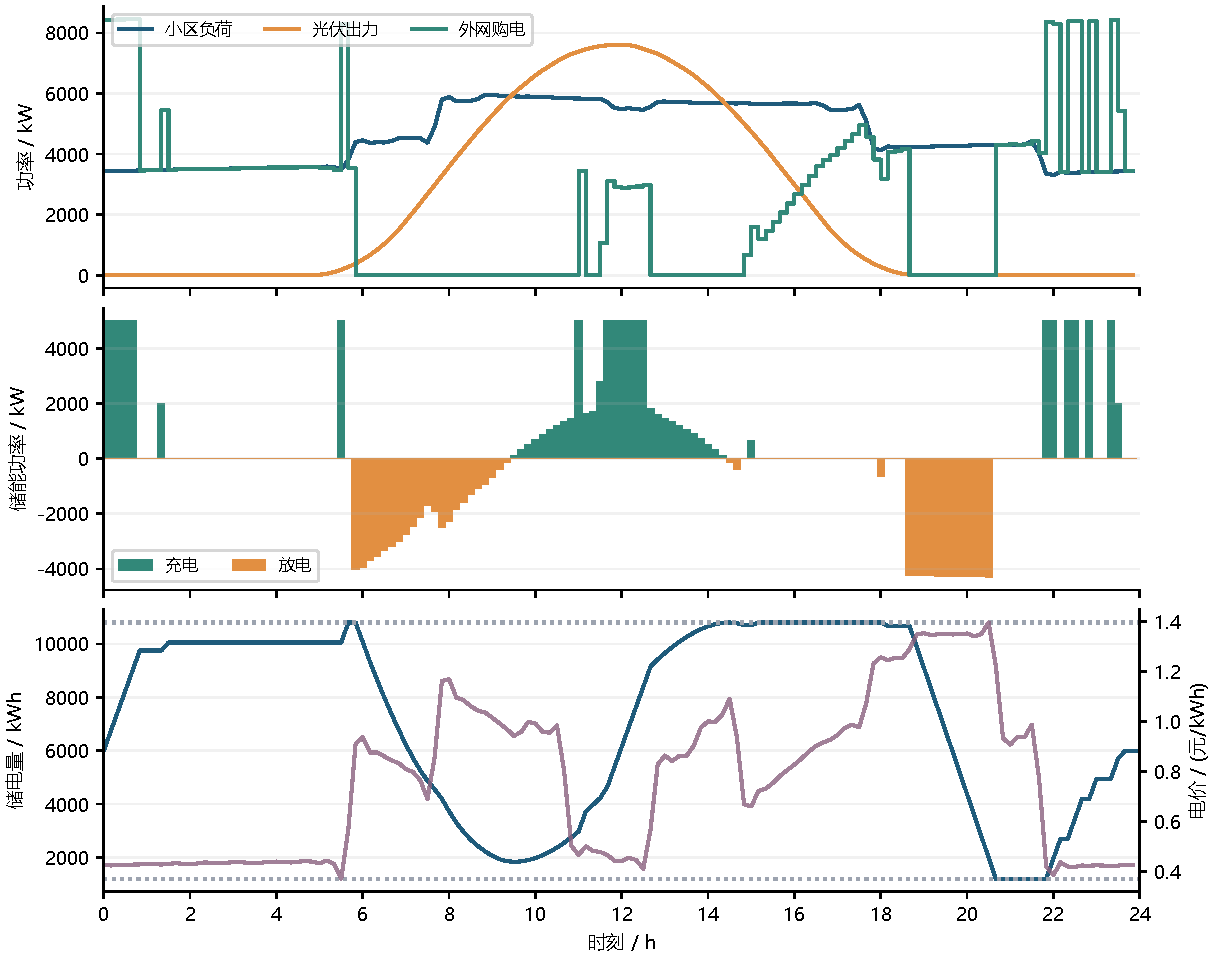
\includegraphics[
    width=0.84\linewidth,
    height=0.60\textheight,
    keepaspectratio
    ]{figures/results/q1_dispatch.pdf}
\caption{问题一购电、充放电、储电量及电价的日内对应关系}
\label{fig:q1}
\end{figure}

图\ref{fig:q1-energy-heatmap}按六个四小时区间标注购电、光伏、负载、充电和放电累计量。平均库存取区间内24段$(e_t+e_{t+1})/2$的均值，并使用独立色标。

\begin{figure}[htbp]\centering
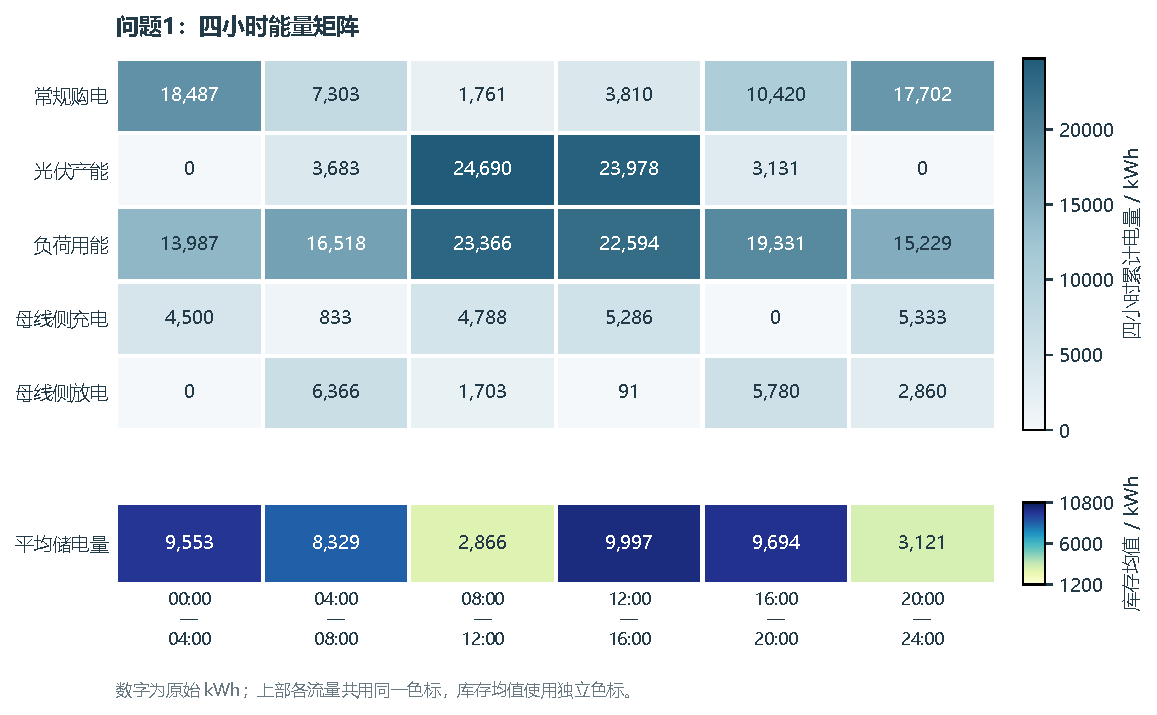
\includegraphics[width=0.88\linewidth]{figures/results/q1_energy_heatmap.pdf}
\caption{问题一六个物理四小时区间的累计电量与平均库存；流量共用色标，库存另设色标，标注单位均为kWh}
\label{fig:q1-energy-heatmap}
\end{figure}
\FloatBarrier
